%----------START object invariant----------

\begin{frame}{HP - Object Invariant}

\vspace*{-0.4cm}

Clusot checks object invariant of the receiver at the end of a
method/constructor and assume it in the pre-state of a call

\vfill

It makes 2 unsound assumptions
\begin{enumerate}
\item assumes invariants of the receiver object in the pre-state of an
instance method
\item assumes the invariant of the receiver after a call to an
inhered method
\end{enumerate}

\end{frame}


\begin{frame}[fragile]{Object Invariant - 1}
\vspace*{-0.4cm}
\only<1>{\lstinputlisting{res/code/objectinvariant1.cs}}
\only<2->{\lstinputlisting{res/code/objectinvariant1assumed.cs}}
\end{frame}


\begin{frame}[fragile]{Object Invariant - 2}
\vspace*{-0.4cm}
\only<1>{\lstinputlisting{res/code/objectinvariant2.cs}}
\only<2->{\lstinputlisting{res/code/objectinvariant2assumed.cs}}
\end{frame}

%----------END object invariant----------
%----------START aliasing----------

\begin{frame}{HP - Aliasing}

\vspace*{-0.4cm}

Clusot unsoundly assumes that heap location not explicitly aliased in the code
analyzed are non-aliasing

\vfill

\begin{textblock*}{1cm}(8.2cm, 4.5cm)
    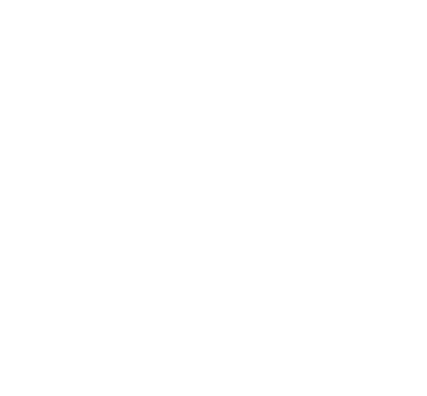
\includegraphics[scale=0.25]{heapgraphexample}
\end{textblock*}

\textbf{Heap graph abstraction}
\lstinputlisting{res/code/heapgraphabstraction.cs}

\end{frame}

\begin{frame}[fragile]{Aliasing}
\vspace*{-0.4cm}
\only<1>{\lstinputlisting{res/code/aliasing.cs}}
\only<2->{\lstinputlisting{res/code/aliasingassumed.cs}}
\end{frame}

%----------END aliasing----------
%----------START write effect----------

\begin{frame}{HP - Write Effect}

\vspace*{-0.6cm}

Clousot uses unsound heuristics to determine the set of heap locations that are
modified by a method call

\vspace*{0.6cm}

It assumes that all other remain unmodified

\vspace*{0.6cm}

This assumption may be not verified in case of aliasing and call to methods
that perform side effects

\end{frame}

\begin{frame}[fragile]{Write Effect}
\vspace*{-0.4cm}
\only<1>{\lstinputlisting{res/code/writeeffect.cs}}
\only<2->{\lstinputlisting{res/code/writeeffectassumed.cs}}
\end{frame}

%----------END write effect----------
%----------START purity----------

\begin{frame}{HP - Purity}

\vspace*{-0.4cm}

Programmers can annotate with \texttt{[Pure]} methods that not make any visible
state changes but \emph{no checks are performed on method purity}

\vspace*{0.6cm}

Clusot unsoundly assumes
\begin{enumerate}
  \item that all method annotated with \texttt{[Pure]} follow the
  specification (as property getters)
  \item that all pure methods deterministically return the same value when
  called in states that are equivalent
\end{enumerate}

\end{frame}


\begin{frame}[fragile]{Purity}
\vspace*{-0.4cm}
\only<1>{\lstinputlisting{res/code/purity1.cs}}
\only<2->{\lstinputlisting{res/code/purity1assumed.cs}}
\end{frame}


% \begin{frame}[fragile]{Purity - 2}
% \vspace*{-0.4cm}
% \only<1>{\lstinputlisting{res/code/purity2.cs}}
% \only<2->{\lstinputlisting{res/code/purity2assumed.cs}}
% \end{frame}

%----------END purity----------